\section{Drive train design}

The following section deals with the design of the drive train and involves the selection of a type of drive train and the calculation of the component specifications therein.

\subsection{Choice of drive train}

The choice of drive train configuration for the wind turbine is made by weighing advantages and disadvantages of various types of typical drive trains and relating them to the market location and desired conditions. A list of advantages and disadvantages of the four most common drive train configurations are listed in Table \ref{tab:comparison_dt}. 

\begin{table}[H]
\hspace*{-2.cm}
\centering
\caption{Comparison of drive train concepts}
\label{tab:comparison_dt}
\begin{tabular}{ |l|l|l|l| }
 \hline
 \textbf{Drivetrain} & \textbf{Advantages} & \textbf{Disadvantages} & \textbf{Specifications} \\ 
 \hline
 Doubly Fed & - Suitable for 2 MW & - Gear failures and & - Pitch control\\ 
  Induction & rated power &  maintenance costs & - For rated\\ 
 (Geared) & - Variable speed & - Generator with & power between\\
  & generator & brushes & 1.5 – 3 MW\\
  & - Active- and & & \\
  & reactive-power control & &\\
  & - Only about a &  & \\
  & third of the power &  & \\
  & flows through inverter & & \\
  & $\to$ smaller inverter & & \\
  & $\to$ lower inverter & & \\
  & cost and losses & & \\
  & - Controlled voltage & & \\
  & and frequency & & \\
  \hline
  Full Conversion & - Good power quality & - Large and heavy & - Pitch control\\
  Permanent Magnet & - Possibility of & - Difficult to transport & For rated power \\
  (Geared on non-) & omitting gearbox & & between 2 – 4 MW \\
  \hline
 Full Conversion High & - Very good & - Complex cooling & - Pitch control\\
 Temperature & power quality & of generator & - For rated power\\
 Superconducting & - Efficient at all loads & - Large torque load & above 5 MW\\
 (Direct Drive) & - Small & & \\
  & - Light & & \\
  & - No gearbox & & \\
  & - Control system can & & \\
  & be adapted to & & \\
  & facilitate operation & & \\
  & on weak grids & & \\
  \hline
  Constant Speed & - Simple design & - Low power quality & - Stall control \\
   & - Lower & - Low control of & - Typically for  \\
   & manufacturing costs & frequency and voltage & rated power below \\
   & & - Narrow range of & 1.5 MW \\
   & & efficient rotational & \\
   & & speed & \\
   & & - Higher cut-in & \\
   & & wind speed & \\
  \hline
 \end{tabular}
\end{table}

\newpage
Although constant speed (CS) drive train turbines have a simple design, due to the lack of speed control systems they have numerous drawbacks that limit their applicability in the Southern African market, even though it makes them cheaper. They produce low power quality as their frequency and voltage is not well controlled, thus requiring a stiff grid. However, particularly in South Africa, the grid is recognisably weak \cite{onishi}. Additionally, CS drive trains are typically used for turbines with a rated power below 1.5 MW, and thus can be ruled out of the options  \cite{mcgahan}.

The full conversion high temperature superconducting (HTS) drive train generates a very good quality power and can be designed small, light and without a gearbox. For these reasons it would be an attractive configuration for Southern Africa where the turbines would have to be transported to the wind farm locations via roads of questionable standards. Nevertheless, full conversion HTS direct drive trains are typically applied for turbines with a rated power above 5 MW and thus can be ruled out as not being suitable for the 2 MW AlphaWind turbine \cite{mcgahan}.

Full conversion permanent magnet (PM) type generators can have direct or geared drive trains and produce good quality power. In cases where no gearbox is used, bulky multipole direct driven generators are used. These are large and thus difficult to transport thus counteracting the benefit of the gear-less configuration \cite{hansen}.

The doubly fed induction generator (DFIG) configuration uses a transmission with a gearbox; however, the output power quality is relatively good as it has a voltage and frequency control. Additionally, the partial frequency converter allows using a smaller and cheaper inverter with lower losses as only about 30\% of the power produced goes through the inverter \cite{hau}. The generator is not particularly bulky as in direct drive trains and can easily be transported to the installation locations. The rated power of the AlphaWind turbine falls well between the range of power for which DFIG is typically applied. Furthermore, considering that power quality and transportability are two very important factors in the choice of drive train for the Southern African region, the DFIG configuration is the most suitable and will thus be applied in the AlphaWind turbine.


\subsection{Gearbox}

\subsubsection{Gearbox summary}

The summary of the gearbox design is given in Table \ref{tab:overview_drivetrain} and \ref{tab:gearbox_config}. 

\begin{table}[h]
\centering
\caption{Overview of the drivetrain}
\label{tab:overview_drivetrain}
\begin{tabular}{ |l|c|c| } 
\hline
\textbf{Parameter} & \textbf{Symbol} & \textbf{Value/Description}\\ 
\hline
Speed range at rated power (LSS / HSS) & $n_{LSS}$/$n_{HSS}$&  14.36 rpm / 1077 rpm \\ 
\hline
Torque at rated power (LSS / HSS) & $Q_{LSS}$ / $Q_{HSS}$ & 1410696 Nm / 18253 Nm\\
\hline
Mass of the gearbox & $m_{gearbox}$ & 17.4 t\\
\hline
\end{tabular} \\
\end{table}

\begin{table}[h]
\centering
\caption{Gearbox configuration}
\label{tab:gearbox_config}
\begin{tabular}{ |l|c|c| } 
\hline
\textbf{Parameter} & \textbf{Symbol} & \textbf{Value/Description}\\ 
\hline
Gearbox type & & 3 stage gearbox\\
\hline
Gearbox stage 1 & & planetary\\
\hline
Gearbox stage 2 & & parallel\\
\hline
Gearbox stage 3 & & parallel\\
\hline
Gearbox ratio & N & 75 \\
\hline
Gear ratio stage 1 & $N_1$ & 5\\
\hline
Gear ratio stage 2 & $N_2$ & 5\\
\hline
Gear ratio stage 3 & $N_3$ & 3\\
\hline
Number of teeth sun& $z_{sun1}$ & 20\\
\hline
Number of teeth planet& $z_{planet3}$ & 30\\
\hline
Number of teeth ring& $z_{ring3}$ & 80\\
\hline
Number of teeth pinion& $z_{p2}$ & 20\\
\hline
Number of teeth gear& $z_{g2}$ & 100\\
\hline
Number of teeth pinion& $z_{p3}$ & 20\\
\hline
Number of teeth gear& $z_{g3}$ & 60\\
\hline
Gearbox length& & 1660 mm\\
\hline
Gearbox diameter& & 2055 mm\\
\hline
\end{tabular} \\
\end{table}

\subsubsection{Supporting material, analyses and rationale}

The torque on the low speed shaft (LSS) needed to generate 2 MW of rated power can be found using the mechanical power on the LSS and the rated angular frequency as
\begin{equation}
    Q_{LSS} = \dfrac{P_{LSS\, rated}}{\omega_{rated}}
    \label{eq:Q_LSS}
\end{equation}
where $P_{LSS}$ is the rated power augmented by the overall drivetrain efficiency. 

The gearbox is designed as a three stages multistage gearbox with the first stage being planetary and the second and third stage being parallel stages. With this an overall gearbox ratio of 75 is achieved. 
The weight of the gearbox is estimated using the following empirical formula

\begin{equation}
    m_{gearbox} = 70.94 \cdot Q_{LSS}^{0.759}
\end{equation}
where $Q_{LSS}$ is the rated LSS torque given by Equation \ref{eq:Q_LSS} inserted in kNm \cite{Fingersh2006}. With this the mass of the gearbox was estimated as

\begin{align}
m_{gearbox} = 17.4 \, t
\end{align}

The gearbox external dimensions, length and diameter, were assumed to be equal to those of a similar DFIG Hitachi 2 MW wind turbine \cite{hitachi}.

\subsection{Generator}

\subsubsection{Generator summary}

The summary of the generator design is given in Table \ref{tab:generator_config}. 
\begin{table}[h]
\centering
\caption{Generator configuration}
\label{tab:generator_config}
\begin{tabular}{ |l|c|c|} 
\hline
\textbf{Parameter} & \textbf{Symbol} & \textbf{Value/Description}  \\ 
\hline
Type of generator & & DFIG\\
\hline
Power rating & & 2.105 MVAr\\
\hline
Generator power factor & pf & 0.95\\
\hline
Grid frequency & $f_{grid}$ & 50 Hz  \\
\hline
Generator poles & $p$ & 6\\
\hline
Generator voltage level & $U_{gen}$ & 1400 V\\
\hline
Generator torque at rated speed & $Q_{HSS}$ & 18253 Nm \\
\hline
Minimum generator speed & $n_{min}$ & 567 rpm\\
\hline
Synchronous speed & $n_s$ & 1000 rpm\\
\hline
Generator rated speed & $n_{rated}$ & 1077 rpm\\
\hline
Maximum generator speed & $n_{max}$ & 1250 rpm \\
\hline
Force density & $F_d$ & 30000 $\frac{N}{m}$\\
\hline
Generator volume & $V_{gen}$ & 0.3042 $m^3$\\
\hline
Generator length & $L_{gen}$ & 1 m\\
\hline
Rotor radius & $R_{rot}$ & 0.3111 m\\
\hline
Rotor mass & $m_{rot}$ & 2388 kg \\
\hline
Generator casing length& & 3538 mm\\
\hline
Generator casing diameter& & 1391 mm\\
\hline
Inertia generator rotor & $\Theta_{rot}$ & 122.5 $kg m^2$\\
\hline
Generator inverter rating & $x$ & 0.25\\
\hline
Safety margin against rotor overshoot & & 16 \%\\
\hline
\end{tabular} \\
\end{table}

\subsubsection{Generator design rationale}

The choice of DIFG for the AlphaWind design offers the advantage to operate at a wide range of generator speeds with high efficiency. The general electrical setup using a DFIG is depicted in Figure \ref{fig:DFIG_figure}. DFIG generators can be operated in voltage control mode (PV) and power factor control mode (PQ) \cite{Londero2012}. Since the turbine is variable speed and thus delivers dependent on the wind speed different amount of power to the grid, the DFIG generator is operated in PV mode with a power factor specified at 0.95. The mechanical power needed to get a desired amount of electrical power out of the turbine is calculated as

\begin{equation}
    P_{in} = \dfrac{P_{out}}{\eta_{el}\eta_{s1}\eta_{s2}\eta_{s3}} + P_{loss\,fix}
    \label{eq:P_in}
\end{equation}
\\
where $\eta_{el}$ is the efficiency of the generator, inverter and all the other components combined (e.g. bearings), $\eta_{si}$ are the efficiencies of the gearbox stages (variable loss) and $P_{loss, \, fix}$ are the fixed losses in the gearbox stages independent of the transmitted power.

\begin{figure}[H]
\centering
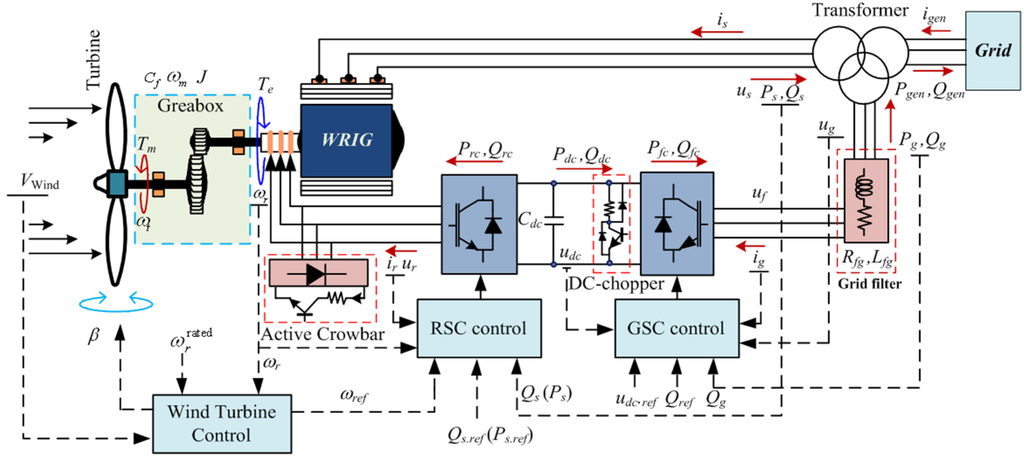
\includegraphics[width=1\textwidth]{Images/DFIG_figure.png} 
\caption{DFIG layout, taken from \cite{Le2016}}
\label{fig:DFIG_figure}
\end{figure}



The the efficiency of the generator together with the bearings is assumed to be constant
\begin{align}
    \eta_{el} = 0.9715
\end{align}

With this the input needed into the generator to produce 2 MW of rated power becomes

\begin{align}
    P_{in\,gen} = \dfrac{P_{rated}}{\eta_{el}} = \dfrac{2 MW}{0.9715} = 2.05 MW
\end{align}

At rated speed each gearbox stage is assumed to have 
loss of transmitted power \cite{hau}. This means an efficiency of $\eta_{ri} = 0.9900$ at rated power for each stage, where half of it is assumed to be independent of the transmitted power and half of it is assumed to be a linear function of the transmitted power. With this the fixed loss of the gearbox is calculated at rated power as half of the sum of the losses in each stage

\begin{align}
    P_{loss\,fix} &= \dfrac{1}{2} \sum \limits_{s = 1}^{3} \left( P_{in} - P_{out}\right)_{s}\\
    &= \dfrac{1}{2} \left( \left( \dfrac{P_{in\,gen}}{\eta_{r1}\eta_{s2} \eta_{r3}} - \dfrac{P_{in\,gen}}{\eta_{r2} \eta_{r3}} \right)_{1} + \left( \dfrac{P_{in\,gen}}{\eta_{r2} \eta_{r3}} - \dfrac{P_{in\,gen}}{\eta_{r3}}\right)_{2}+ \left( \dfrac{P_{in\,gen}}{\eta_{r3}} - P_{in\,gen} \right) \right)\\
    &= \dfrac{1}{2} \left( \dfrac{2.05 MW}{0.99^3} - 2.05 MW \right) = 31.5 \,kW
\label{eq:Ploss_fix}
\end{align}

For the losses that vary with the power in Equation \ref{eq:P_in} subsequently a gearbox efficiency of $\eta_{si} = 0.9950$ must be used (since the fixed 0.5 \% loss is accounted via $P_{loss \, fix}$).

\newpage
With this the overall efficiency of the drivetrain at rated power is

\begin{align}
\eta_{tot, rated} = 0.9430    
\end{align}

The dimensions of the generator rotor are calculated using the formulae given in the lecture. We assume the flux density of the stator windings to be $F_d = 30000 \frac{N}{m}$. With this volume of the rotor is calculated as

\begin{equation}
    V_{rot} = \dfrac{P_{in \, gen}}{2 \omega_{rated} F_d} = \dfrac{2.05 MW}{2 \cdot 112.78 \frac{rad}{s} \cdot 30000 \frac{N}{m}} = 0.3042 \,m^3
\end{equation}

The length of the generator rotor was assumed to be 1 m, with this the generator rotor radius $R_{rot}$ was calculated. Using these dimensions the generator rotor mass is estimated. The overall generator mass (rotor + stator + housing) is calculated using again the empirical formula given in Reference~\cite{Fingersh2006}

\begin{equation}
    m_{generator} = 6.47 \left(P_{rated}\right)^{0.9223}
\end{equation}

where $P_{rated}$ is the rated power of the turbine inserted in kW. 

The generator rotor inertia is calculated using the standard formula for the inertia of a rotor

\begin{align}
\Theta_{rot} &= \dfrac{1}{2}m_{rot}R_{rot}^2 \\
&= \dfrac{1}{2}\cdot 2388\,kg \cdot (0.3111 \,m)^2 = 122.5 \, kgm^2 \nonumber
\end{align}

The generator inverter rating, $x$, is used to specify the minimum speed of the generator that is required to start it. This speed is obtained as

\begin{equation}
    \omega_{cut-in} = \dfrac{(1- \sqrt{3}\cdot x)\cdot n_s}{N}= 7.56\ rpm
\label{eq:cut-in_speed}
\end{equation}

where $x$ is the generator inverter rating, $n_s$ is the synchronous speed and $N$ is the gear-box ratio of the drivetrain. 
The power lost in the gearbox, given by Equation \ref{eq:Ploss_fix}, needs to be overcome by the rotor at the cut-in wind speed and the cut-in rotational speed, to be able to move the rotor and simultaneously start the generator. The value of the cut-in rotational speed obtained for the rotor is used to calculate the cut-in wind velocity, $v_{cut-in}$, at which the rotor will just overcome the resistance provided by the drive-train and thus start motion. This is done by using the $C_p-\lambda$ curve at a rotational speed of $\omega_{cut-in}$ in order to obtain the wind velocity at which the power losses in the gear-box can be overcome.
In the relation for the tip-speed ratio given by $\lambda= \frac{\omega_{cut-in} R}{v}$, the tip-speed ratio is varied by varying the wind velocity $v$. The power coefficient, $C_p$, is then calculated for each tip-speed ratio. Using this value the power is obtained for each of the wind velocity value used to calculate the tip-speed ratio. The corresponding velocity at which the fixed losses in the gear-box, given by Equation \ref{eq:Ploss_fix}, are overcome, is then chosen as the cut-in wind velocity.
The cut-in wind velocity, $v_{cut-in}$, is thus obtained as

\begin{equation}
    v_{cut-in} = 3\ m/s
\label{eq:cut-in_wind_vel}
\end{equation}

The generator casing dimensions, length and diameter, were assumed to be equal to those of a similar DFIG Hitachi 2 MW wind turbine \cite{hitachi}.


\begin{figure}[H]
\centering
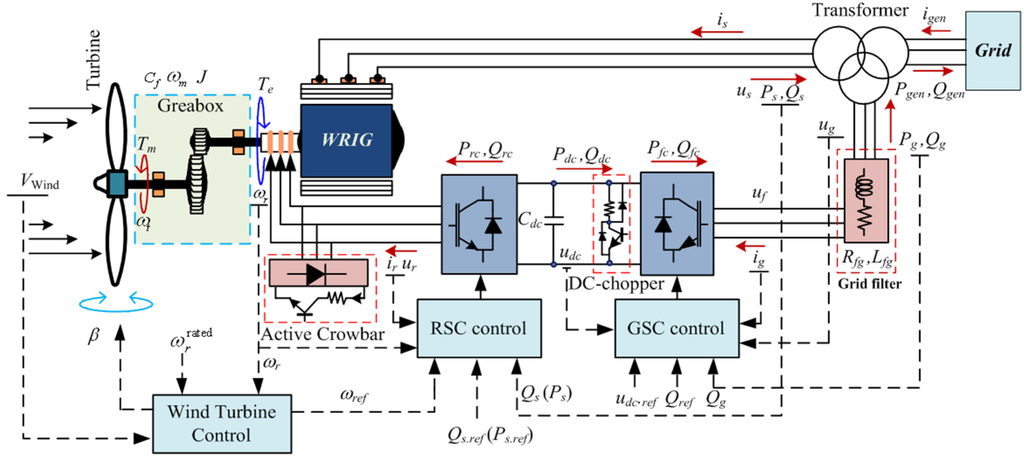
\includegraphics[width=1\textwidth]{Images/DFIG_figure.png} 
\caption{Power curve of AlphaWind Turbine}
\label{fig:power_curve}
\end{figure}


\newpage
\subsection{Inverter}

\subsubsection{Inverter summary}

\begin{table}[h]
\centering
\caption{Specification of ACS800-67 inverter}
\label{tab:inverter}
\begin{tabular}{ |l|c|c|} 
\hline
\textbf{Parameter} & Symbol & \textbf{Value/Description} \\ 
\hline
Type of converter & & Air cooled doubly-fed converter \\
\hline
Inverter voltage level & $U$ & up to 12 kV\\
\hline
Generator nominal power range & & 0.9 - 2.2 MW \\
\hline
Efficiency at rated power & & 98 \% \\ 
\hline
Nominal frequency & $f$ & 50 Hz $\pm 3$ \% \\
\hline
Location of the converter & & tower base  \\ 
\hline
Dimensions of cabinet & W & 2500 mm \\
\hline
& H & 1800 mm \\
\hline
& D & 600 mm \\
\hline
Weight of inverter & $m_{inverter}$ & 1900 kg \\
\hline
\end{tabular} \\
\end{table}


\subsubsection{Choice of inverter and design}

As inverter the ACS800-67 conveter by ABB is chosen \cite{ABB}. The generator voltage level is chosen at the upper limit specified by the manufacturer for the inverter. According to ABB the inverter can operate at to 12 kV, so this voltage is chosen. With this the currents per phase in the cables connecting the generator with the inverter at the bottom of the tower can be reduced, which reduces the copper losses of the electrical transmission. Nowadays most turbine manufacturers locate the inverter cabinet at the base of the tower, including it's cooling system which is also located in the tower \cite{hau}.

\subsection{Power cables}

\subsubsection{Cables summary}
The summary of the cable design is given in Table \ref{tab:power_cables}.

\begin{table}[h]
\centering
\caption{Power cables in tower}
\label{tab:power_cables}
\begin{tabular}{ |l|c|c|} 
\hline
\textbf{Parameter} & Symbol & \textbf{Value/Description}  \\ 
\hline
Voltage level & $U$ & 12 kV\\
\hline
Current per phase & $I_{phase}$ & 101.3 A\\
\hline
Cable & & TECWIND(H) (N)TSCGEHXOEU 5DK9 501  \\
\hline
Cable approval & & DIN VDE 0250, Part 813 \\
\hline
\end{tabular} \\
\end{table}

\subsubsection{Cable selection}

The cable chosen for inside the turbine tower is the (N)TSCGEHXOEU cable by Draka Industry\&Speciality. This three phase cable with Copper cores is specially designed for application in Wind Turbines and certified for  Uo/U = 3.6/6.0 kV to 20/35 kV at 50 Hz \cite{Draka}. This cable is chosen because of it's high flexibility which is needed inside the tower to connect the yawed turbine nacelle to the inverter at the bottom of the tower.

The current per phase is calculated as

\begin{align}
    I_{phase} &= \dfrac{P_{rated}}{\sqrt{3}U \cos \phi} \\
    &= \dfrac{2 MW}{\sqrt{3} \cdot 12 kV \cdot 0.95} = 101.3\,A \nonumber
\end{align}

To connect with the grid the generator stator is directly connected to the transformer station outside the tower and the generator rotor is connected to the inverter which is located at the bottom of the wind turbine tower. Therefore two cable strings of 3 phase power cable are needed inside the tower. With the hub height being 70.36 m the overall cable length from generator to the inverter is estimated to be 160 m. 

The copper losses for all three phases at rated power can be estimated as

\begin{align}
    P_{loss} &= 3 \rho I_{phase}^2 L_{cable} \\
    &= 3 \cdot 0.000672\,Ohm/m \cdot \left(101.3\,A\right)^2 \cdot 160\,m = 3.3\,kV \nonumber
\end{align}

where $\rho$ is the specific resistance of the copper cable that is being calculated using the conductivity of copper and the cross sectional surface of 25 $mm^2$ per phase. 

\subsection{Diagram of drive train configuration}

Figure \ref{fig:eddie's art} shows a schematic two dimensional diagram of the nacelle and the tower base in which the designed components are to scale with respect to each other, the nacelle and the tower diameter. The length and diameter of the gearbox and generator are those specified in tables \ref{tab:gearbox_config} and \ref{tab:generator_config}. The nacelle dimensions are assumed to be the same as those of a similar DFIG Hitachi 2 MW wind turbine with a length of 6.7 m and a height of 4 m \cite{hitachi}. The tower base diameter of 4.76 m has been obtained by scaling from the reference turbine. The inverter dimensions are those specified in table \ref{tab:inverter}. The tilt angle of the shaft is of $5\deg$ which is the same as the reference turbine.


\begin{figure}[H]
    \centering
    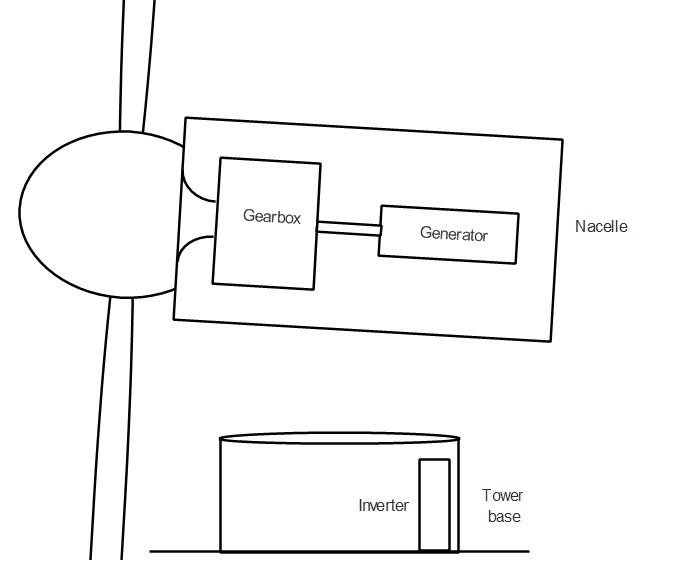
\includegraphics[width=1\textwidth]{Images/Drive_train_sketch.jpg}
    \caption{Schematic diagram of drive train configuration}
    \label{fig:eddie's art}
\end{figure}


